\documentclass[preprint,12pt,3p]{elsarticle}

\usepackage{amsmath,amssymb,amsfonts,amsthm}
\usepackage{booktabs}
\usepackage{multirow}
\usepackage{graphicx}
\usepackage{algorithm}
\usepackage{algorithmic}
\usepackage{hyperref}
\usepackage{cleveref}
\usepackage{tikz}
\usetikzlibrary{shapes,arrows,positioning}

\journal{Knowledge-Based Systems}

\newtheorem{theorem}{Theorem}
\newtheorem{definition}{Definition}
\newtheorem{assumption}{Assumption}

\begin{document}

\begin{frontmatter}

\title{Diff-GNN-Bandit: Generative Score-Based Diffusion and Causal Graph Reinforcement Learning for Safe Offline Policy Optimization}

\author{Zarif Latif\corref{cor1}}
\ead{zariffromlatif@gmail.com}
\cortext[cor1]{Corresponding author}

\begin{abstract}
Customer retention and personalized intervention optimization are pivotal challenges in contemporary digital enterprise systems. Traditional retention frameworks rely predominantly on supervised churn prediction, identifying at-risk users while failing to prescribe actionable, causal interventions that maximize customer lifetime value. While offline reinforcement learning (RL) and contextual bandits provide formal foundations for counterfactual decision-making, their practical deployment is obstructed by two systemic barriers: (1) severe state-action sparsity and cold-start regimes where individual interaction histories are sparse or absent, and (2) catastrophic out-of-distribution (OOD) extrapolation errors induced by distributional shift between the historical logging policy and learned target policies. In this paper, we propose \textbf{Diff-GNN-Bandit}, a unified framework uniting Graph Neural Networks, Batch-Constrained Reinforcement Learning, and Score-Based Generative Diffusion Policies for safe offline policy optimization. GNN-Bandit constructs a bipartite user-item relational interaction graph and utilizes a non-linear-free Graph Convolutional Network (LightGCN) to diffuse treatment-response signals across multi-hop collaborative neighborhoods. We establish that this linear propagation operates as an adaptive low-pass graph spectral filter, preserving low-frequency homophilic causal signals while attenuating observational noise, thereby enabling robust inductive generalization to zero-degree cold-start users. To eliminate out-of-distribution extrapolation errors without discrete support truncation pathologies, we formulate policy generation as a continuous score-based diffusion process operating directly in the latent item embedding manifold, steered at inference time by closed-form analytical Tweedie CATE guidance gradients. We also formulate offline policy optimization and enterprise budget allocation through the lens of Lagrangian duality, proving that batch constraints and counterfactual variance bounds emerge naturally as primal-dual solutions under bounded risk. We conduct extensive empirical evaluations across six large-scale benchmark datasets comprising more than 40 million logged interactions from the Open Bandit Dataset (OBD-All, Men, Women), the Criteo Uplift benchmark, and large-scale micro-video platforms (KuaiRec, KuaiRand), benchmarking against 11 competitive baselines. Off-policy evaluation via Doubly Robust (DR) estimation demonstrates that GNN-Bandit attains the highest policy value on all three OBD campaigns, outperforming the strongest baseline by \textbf{+25.31\% on OBD-All} ($p = 1.2 \times 10^{-5}$), \textbf{+16.08\% on OBD-Men} ($p = 7.8 \times 10^{-4}$), and \textbf{+17.28\% on OBD-Women} ($p = 0.0018$) across five random seeds, while surpassing the historical logging policy on every benchmark (+13.50\% to +107.50\%). On KuaiRand, our score-based diffusion policy equipped with Tweedie CATE guidance achieves a highly significant $+1.99\%$ DR lift ($p = 1.93 \times 10^{-5}$) over unguided diffusion with sub-3 microsecond real-time inference latency. In zero-degree cold-start partitions, GNN-Bandit achieves up to \textbf{+42.87\%} lift over matrix factorization baselines. Diff-GNN-Bandit establishes an empirically validated and theoretically grounded blueprint for high-stakes offline decision support.
\end{abstract}

\begin{keyword}
Diffusion Models \sep Score-Based Generative Policies \sep Graph Neural Networks \sep Offline Reinforcement Learning \sep Batch-Constrained Policy Optimization \sep Causal Uplift Modeling \sep Lagrangian Duality \sep Off-Policy Evaluation.
\end{keyword}

\end{frontmatter}

\section{Introduction}
\label{sec:intro}

In modern digital economies, customer churn represents one of the most substantial threats to enterprise profitability and sustainable growth. Acquiring a new customer is widely documented to cost five to seven times more than retaining an existing one. Consequently, commercial platforms dedicate extensive computational resources to proactive customer retention and personalized engagement systems.

However, existing industrial practice predominantly suffers from a fundamental conceptual mismatch: \textbf{predictive modeling is conflated with prescriptive intervention}. Standard machine learning approaches frame customer retention as a supervised classification task---predicting the probability that a user will churn within a future observation window. While predictive models can accurately identify high-churn-risk individuals, they provide zero insight into \textit{which intervention} (e.g., promotional discount, targeted recommendation, feature highlight, or no contact) will causally alter that user's trajectory. Treating all high-risk users indiscriminately frequently leads to severe marketing inefficiencies:
\begin{enumerate}
    \item \textbf{Wasted Expenditure on ``Sure Things''}: Users who would remain active regardless of intervention receive costly incentives.
    \item \textbf{Harm to ``Sleeping Dogs''}: Users who are content in a dormant state are annoyed or prompted to cancel their subscriptions upon receiving unsolicited outreach (negative treatment effect).
    \item \textbf{Neglect of ``Persuadables''}: Users whose retention decisions are highly sensitive to specific, tailored recommendations are overlooked because their baseline churn risk may be moderate.
\end{enumerate}

To transition from passive prediction to prescriptive decision-making, the problem must be formalized as a \textbf{contextual bandit} or \textbf{offline reinforcement learning (RL)} problem. In this paradigm, a decision agent observes user context $\mathbf{x}$, selects an action $a \in \mathcal{A}$, and observes a feedback reward $r \in \{0, 1\}$.

Deploying online RL agents directly in production is unacceptable in high-stakes commercial environments due to the catastrophic revenue loss and customer dissatisfaction caused by exploratory, sub-optimal actions. Platforms must therefore learn exclusively from \textbf{offline logged interaction datasets} $\mathcal{D}_0 = \{(x_i, a_i, r_i, p_i)\}_{i=1}^N$ collected by historical logging policies $\pi_0$. Offline policy optimization under logging bias introduces two severe methodological hurdles:
\begin{enumerate}
    \item \textbf{Distributional Shift and Extrapolation Error}: Standard value-based RL algorithms greedily maximize $Q(s, a)$ over all actions. For unobserved state-action pairs ($a \notin \text{supp}(\pi_0(\cdot|s))$), neural network function approximators produce unchecked over-optimistic value estimates. When the learned policy selects these out-of-distribution (OOD) actions, real-world deployment fails catastrophically.
    \item \textbf{Extreme Sparsity and the Cold-Start Dilemma}: Real-world user populations exhibit power-law interaction topologies. In the Open Bandit Dataset (OBD), for example, 51.8\% of user segments (249 of 481) are complete \textbf{cold-start nodes} with zero prior positive interactions. Standard Euclidean feature representations fail because isolated feature vectors contain insufficient signal to infer personalized causal responsiveness.
\end{enumerate}

To simultaneously resolve distributional shift, cold-start relational sparsity, and enterprise operational constraints, we introduce \textbf{GNN-Bandit}, a unified Graph-Enhanced Causal Reinforcement Learning framework:
\begin{itemize}
    \item \textbf{Topological Causal Smoothing}: We construct a bipartite interaction graph $\mathcal{G} = (\mathcal{U}, \mathcal{I}, \mathcal{E})$ and leverage LightGCN \cite{he2020lightgcn} to perform linear graph convolutions without non-linear feature distortion. This acts as a low-pass graph spectral filter, propagating treatment-response signals across multi-hop collaborative neighborhoods and providing rich inductive priors for cold-start users.
    \item \textbf{Batch-Constrained Safety Filtering}: We implement a state-conditioned action plausibility filter $\hat{\mathcal{A}}(s)$ driven by a behavioral cloning network $\hat{P}_\beta(a|s)$. The agent is mathematically restricted to actions that have demonstrated historical logging support, strictly eliminating OOD counterfactual extrapolation errors.
    \item \textbf{Lagrangian Duality and Budget Pacing}: We formulate offline policy constraints and real-world marketing budget limitations as a constrained optimization problem, demonstrating how the BCQ action filter and counterfactual variance bounds emerge naturally from Lagrangian relaxation.
    \item \textbf{Risk-Averse Quantile Optimization (CVaR)}: We employ distributional quantile regression to estimate the Conditional Value-at-Risk ($\text{CVaR}_\alpha$) of candidate interventions, allowing decision-makers to tune the policy along a formal safety-performance Pareto frontier.
    \item \textbf{Generative Diffusion Policy \& Tweedie CATE Guidance (Diff-GNN-Bandit)}: To scale to continuous latent action representations and large catalogs, we formulate action generation as a score-based diffusion process over graph embeddings. We derive an analytical closed-form Tweedie CATE guidance gradient that steers policy trajectories toward high-uplift decisions at inference time in $<3\ \mu\text{s}$ without neural backpropagation or model retraining.
    \item \textbf{Doubly Robust Off-Policy Validation}: Policy performance is verified via Doubly Robust (DR) estimation across six real-world datasets, guaranteeing consistent and asymptotic variance-reduced evaluation without live environmental exposure.
\end{itemize}

\section{Problem Formulation \& Theoretical Foundations}
\label{sec:problem}

\subsection{Offline Contextual Bandit Setup}
Let $\mathcal{M} = (\mathcal{X}, \mathcal{A}, \mathcal{R}, \mathcal{P}, \pi_0)$ define an offline contextual bandit environment under batch logging constraints:
$\mathcal{X} \subseteq \mathbb{R}^d$ denotes the user context space; $\mathcal{A} = \{a_1, a_2, \dots, a_K\}$ denotes the finite discrete action space; $\mathcal{R}: \mathcal{X} \times \mathcal{A} \to [0, 1]$ represents the stochastic reward distribution with expectation $r(x, a) = \mathbb{E}[r \mid x, a]$; and $\pi_0(a \mid x)$ denotes the stochastic logging policy that collected dataset $\mathcal{D}_0 = \{ (x_i, a_i, r_i, p_i) \}_{i=1}^N$ with propensity $p_i = \pi_0(a_i \mid x_i)$. The objective is to find a target policy $\pi: \mathcal{X} \to \Delta(\mathcal{A})$ maximizing the expected counterfactual return:
\begin{equation}
V(\pi) = \mathbb{E}_{x \sim \mathcal{P}, a \sim \pi(\cdot \mid x)} \left[ r(x, a) \right] = \int_{\mathcal{X}} \sum_{a \in \mathcal{A}} \pi(a \mid x) r(x, a) \mathcal{P}(x) \, dx
\end{equation}

\subsection{Causal Potential Outcomes \& Uplift Identification}
Following the Neyman-Rubin potential outcomes framework, let $Y(a) \in \{0, 1\}$ denote the potential outcome had action $a$ been assigned. The Conditional Average Treatment Effect (CATE) relative to baseline control $a_0$ is:
\begin{equation}
\tau_{\mathrm{CATE}}(x, a) = \mathbb{E}[Y(a) - Y(a_0) \mid X = x] = \mu(x, a) - \mu(x, a_0)
\end{equation}
Under the standard causal assumptions of Stable Unit Treatment Value (SUTVA), Unconfoundedness ($\{Y(a)\} \perp A \mid X$), and Positivity ($\pi_0(a \mid x) \ge \epsilon > 0$), $\tau_{\mathrm{CATE}}$ is non-parametrically identifiable. The target policy seeks to concentrate intervention probability on the \textit{Persuadables} quadrant ($\tau > 0$) while strictly suppressing actions on \textit{Sleeping Dogs} ($\tau < 0$).

\subsection{Graph Representation Theory \& Spectral Smoothing}
Let $\mathcal{G} = (\mathcal{V}, \mathcal{E})$ denote the bipartite interaction graph with adjacency matrix $\mathbf{A} \in \mathbb{R}^{(N_u + N_i) \times (N_u + N_i)}$:
\begin{equation}
\mathbf{A} = \begin{bmatrix} \mathbf{0} & \mathbf{R} \\ \mathbf{R}^\top & \mathbf{0} \end{bmatrix}
\end{equation}
where $\mathbf{R} \in \mathbb{R}^{N_u \times N_i}$ represents historical positive interactions. Let $\tilde{\mathbf{A}} = \mathbf{D}^{-1/2} \mathbf{A} \mathbf{D}^{-1/2}$ be the symmetrically normalized adjacency matrix. LightGCN performs layer-wise linear aggregation:
\begin{equation}
\mathbf{E}^{(k+1)} = \tilde{\mathbf{A}} \mathbf{E}^{(k)}, \quad \mathbf{E}^* = \sum_{k=0}^L \alpha_k \mathbf{E}^{(k)}, \quad \alpha_k = \frac{1}{L + 1}
\end{equation}

\begin{theorem}[Low-Pass Causal Spectral Filtering]
Let $\mathbf{L}_{\mathrm{sym}} = \mathbf{I} - \tilde{\mathbf{A}} = \mathbf{U} \mathbf{\Lambda} \mathbf{U}^\top$ denote the eigendecomposition of the normalized graph Laplacian with eigenvalues $\lambda_m \in [0, 2]$. The $L$-layer LightGCN operator acts as a spectral polynomial filter $g(\lambda) = \sum_{k=0}^L \alpha_k (1 - \lambda)^k$.
\end{theorem}
\begin{proof}
For an input signal $\mathbf{x} \in \mathbb{R}^{|\mathcal{V}|}$, the $k$-th diffusion step is $\tilde{\mathbf{A}}^k \mathbf{x} = (\mathbf{I} - \mathbf{L}_{\mathrm{sym}})^k \mathbf{x} = \mathbf{U} (\mathbf{I} - \mathbf{\Lambda})^k \mathbf{U}^\top \mathbf{x}$. Summing over all layers $k \in \{0, \dots, L\}$ with weights $\alpha_k$:
\begin{equation}
\mathbf{E}^* = \sum_{k=0}^L \alpha_k \tilde{\mathbf{A}}^k \mathbf{E}^{(0)} = \mathbf{U} \left( \sum_{k=0}^L \alpha_k (\mathbf{I} - \mathbf{\Lambda})^k \right) \mathbf{U}^\top \mathbf{E}^{(0)} = \mathbf{U} g(\mathbf{\Lambda}) \mathbf{U}^\top \mathbf{E}^{(0)}
\end{equation}
Since $g(\lambda) = \frac{1}{L+1} \sum_{k=0}^L (1 - \lambda)^k$ is strictly monotonically decreasing on $\lambda \in [0, 2]$ with $g(0) = 1$ and $g(2) \approx 0$, high-frequency graph noise is attenuated while low-frequency homophilic causal response signals are smoothed across collaborative neighbors.
\end{proof}

\begin{lemma}[Graph Convolutional Contraction of Representation IPM]
\label{lem:ipm_contraction}
Let $\mathcal{P}_X$ and $\mathcal{Q}_X$ denote the feature distributions of treated and control populations over bipartite graph $\mathcal{G} = (\mathcal{U} \cup \mathcal{I}, \mathcal{E})$. Let $\Phi(X) = \mathbf{U} g(\mathbf{\Lambda}) \mathbf{U}^\top X$ denote the representation obtained via the layer-averaged LightGCN operator $g(\mathbf{\Lambda}) = \frac{1}{L+1} \sum_{k=0}^L (\mathbf{I} - \mathbf{\Lambda})^k$. Under the family of 1-Lipschitz test functions $\mathcal{F} = \{f : \|f\|_{\mathrm{Lip}} \le 1\}$, the Integral Probability Metric (IPM) contracts geometrically on the non-trivial spectral subspace:
\begin{equation}
\mathrm{IPM}_{\mathcal{F}}(\mathcal{P}_{\Phi}, \mathcal{Q}_{\Phi}) \le (1 - \lambda_2(\mathbf{L}_{\mathrm{sym}}))^L \cdot \mathrm{IPM}_{\mathcal{F}}(\mathcal{P}_X, \mathcal{Q}_X)
\end{equation}
where $\lambda_2(\mathbf{L}_{\mathrm{sym}}) > 0$ is the spectral gap (Fiedler eigenvalue) of the normalized graph Laplacian. Furthermore, for odd layer depth $L$ (such as $L=3$), the bipartite boundary alternating mode at $\lambda_N = 2$ is identically annihilated ($g(2) = 0$).
\end{lemma}
\begin{proof}
By the Kantorovich-Rubinstein duality theorem, $\mathrm{IPM}_{\mathcal{F}}(\mathcal{P}, \mathcal{Q}) = \mathcal{W}_1(\mathcal{P}, \mathcal{Q})$. On a bipartite graph, the normalized adjacency spectrum is symmetric: $\mu_1 = 1$ and $\mu_N = -1$ (corresponding to Laplacian eigenvalues $\lambda_1 = 0$ and $\lambda_N = 2$). The polynomial spectral filter satisfies $g(\lambda) = \frac{1}{L+1}\sum_{k=0}^L (1 - \lambda)^k$. For odd $L$, $g(2) = \frac{1}{L+1}\sum_{k=0}^L (-1)^k = 0$, completely suppressing bipartite alternating noise. On the non-trivial homophilic spectrum $\lambda \in [\lambda_2, 2 - \lambda_2]$, the operator norm is bounded by the spectral radius $\rho \le 1 - \lambda_2(\mathbf{L}_{\mathrm{sym}})$. For any $f \in \mathcal{F}$, $\|f \circ g(\tilde{\mathbf{A}})\|_{\mathrm{Lip}} \le (1 - \lambda_2)^L \|f\|_{\mathrm{Lip}}$. Taking the supremum over $\mathcal{F}$ yields the geometric contraction bound.
\end{proof}

\begin{theorem}[Finite-Sample PEHE Generalization Error Bound]
\label{thm:pehe_bound}
Let $\hat{\tau}(x) = h_1(\Phi(x)) - h_0(\Phi(x))$ be the estimated CATE function parameterized by hypotheses $h_0, h_1 \in \mathcal{H}$ over graph representations $\Phi(X)$. With probability at least $1 - \delta$ over the random draw of $N$ offline logged transitions:
\begin{equation}
\mathrm{PEHE}(\hat{\tau}) \le 2 \left( \hat{\epsilon}_{\mathrm{factual}} + 2 \mathcal{R}_N(\mathcal{H}) + c \sqrt{\frac{\log(2/\delta)}{N}} \right) + 2 L_h (1 - \lambda_2)^L \cdot \mathrm{IPM}_{\mathcal{F}}(\mathcal{P}_X, \mathcal{Q}_X)
\end{equation}
where $\mathcal{R}_N(\mathcal{H})$ is the empirical Rademacher complexity of the hypothesis class $\mathcal{H}$, $L_h$ is the Lipschitz constant of the regression heads, and $\mathrm{PEHE}(\hat{\tau}) = \int_{\mathcal{X}} (\hat{\tau}(x) - \tau(x))^2 \mathcal{P}(x) dx$.
\end{theorem}
\begin{proof}
Decomposing the Precision in Estimating Heterogeneous Effects (PEHE) into factual prediction error and counterfactual domain discrepancy follows Shalit et al. \cite{shalit2017estimating}. Applying Lemma~\ref{lem:ipm_contraction} bounds the domain discrepancy by $(1 - \lambda_2)^L \mathrm{IPM}_{\mathcal{F}}(\mathcal{P}_X, \mathcal{Q}_X)$, while standard empirical process theory bounds the factual error using Rademacher complexity $\mathcal{R}_N(\mathcal{H})$ and McDiarmid's concentration inequality.
\end{proof}

\begin{theorem}[Offline Policy Suboptimality Bound under Graph BCQ]
\label{thm:bcq_subopt}
Let $\pi^*$ denote the optimal unconstrained counterfactual policy, and let $\hat{\pi}_{\mathrm{BCQ}}$ be the policy learned by GNN-Bandit under batch constraint threshold $\tau$. The counterfactual policy value suboptimality is bounded by:
\begin{equation}
V(\pi^*) - V(\hat{\pi}_{\mathrm{BCQ}}) \le 2 \epsilon_{\mathrm{extrap}}(\tau) + \mathcal{O}\left( \sqrt{\frac{d_{\mathcal{H}} \log(N)}{N}} \right) + (1 - \beta) \sqrt{\mathrm{PEHE}(\hat{\tau})}
\end{equation}
where $\epsilon_{\mathrm{extrap}}(\tau) = \max_{s} \max_{a \notin \hat{\mathcal{A}}(s)} [Q^*(s, a) - \max_{a' \in \hat{\mathcal{A}}(s)} Q^*(s, a')]_+$ is the out-of-support truncation loss, and $d_{\mathcal{H}}$ is the pseudo-dimension of the Q-network.
\end{theorem}
\begin{proof}
The policy suboptimality decomposes into out-of-support action truncation error $\epsilon_{\mathrm{extrap}}(\tau)$, sample complexity bounded by empirical VC/Rademacher dimensions $\mathcal{O}(\sqrt{d_{\mathcal{H}} \log(N)/N})$, and CATE reward augmentation error scaled by $(1 - \beta)\sqrt{\mathrm{PEHE}(\hat{\tau})}$. In the single-step contextual bandit setting ($\gamma = 0$), the standard sequential error amplification factor $\frac{2}{1 - \gamma}$ reduces identically to 2. When logging support is dense on the optimal action, $\epsilon_{\mathrm{extrap}}(\tau) = 0$, guaranteeing near-optimal generalization.
\end{proof}


\section{Proposed Methodology: GNN-Bandit}
\label{sec:method}

\subsection{Lagrangian Formulation of Constrained Offline Policy Optimization}
To prevent distributional shift, the offline policy optimization problem is formulated as:
\begin{equation}
\max_{\pi \in \Pi} \; \mathbb{E}_{x \sim \mathcal{P}, a \sim \pi(\cdot \mid x)} \left[ Q(x, a) \right] \quad \text{s.t.} \quad \mathbb{E}_{x \sim \mathcal{P}} \left[ D_{\mathrm{KL}}\Big( \pi(\cdot \mid x) \;\big\|\; \pi_0(\cdot \mid x) \Big) \right] \le \epsilon
\end{equation}
Introducing the Lagrange multiplier $\lambda \ge 0$, the unconstrained minimax objective is:
\begin{equation}
\max_{\pi} \min_{\lambda \ge 0} \; \mathcal{L}(\pi, \lambda) = \mathbb{E}_{x} \left[ \sum_{a \in \mathcal{A}} \pi(a \mid x) Q(x, a) \right] - \lambda \left( \mathbb{E}_{x} \left[ D_{\mathrm{KL}}(\pi(\cdot \mid x) \,\|\, \pi_0(\cdot \mid x)) \right] - \epsilon \right)
\end{equation}
Under strong duality, the optimal solution for a fixed multiplier $\lambda > 0$ is the regularized Gibbs policy $\pi^*(a \mid x) \propto \pi_0(a \mid x) \exp(Q(x, a)/\lambda)$. Batch-Constrained Q-learning (BCQ) corresponds to the non-parametric limit: actions with insufficient logging support ($\pi_0(a \mid x) < \tau$) are assigned an infinite Lagrangian penalty ($\lambda \to \infty$), zeroing their probability mass and eliminating OOD extrapolation error.

\subsection{Budget-Constrained Retention via Lagrangian Relaxation}
When interventions incur cost $c(x, a)$ under total budget $B$, the problem becomes:
\begin{equation}
\max_{\pi} \sum_{i=1}^N \mathbb{E}\left[ r(x_i, \pi(x_i)) \right] \quad \text{s.t.} \quad \sum_{i=1}^N c(x_i, \pi(x_i)) \le B
\end{equation}
The Lagrangian relaxation introduces the shadow price $\lambda_{\mathrm{cost}} \ge 0$:
\begin{equation}
\mathcal{L}_{\mathrm{budget}}(\pi, \lambda_{\mathrm{cost}}) = \sum_{i=1}^N \left( \mathbb{E}\left[ r(x_i, \pi(x_i)) \right] - \lambda_{\mathrm{cost}} c(x_i, \pi(x_i)) \right) + \lambda_{\mathrm{cost}} B
\end{equation}
This establishes that under capital constraints, optimal policy intervention occurs exclusively when the marginal uplift-to-cost ratio satisfies $\frac{\tau_{\mathrm{CATE}}(x, a)}{c(x, a)} \ge \lambda_{\mathrm{cost}}$.

\subsection{Quantile Q-Learning and CVaR Risk-Sensitive Objective}
We estimate the return distribution via Quantile Regression with $M$ quantiles $\theta_m(s, a)$, trained using the Huber quantile loss at target quantiles $\xi_m = \frac{2m - 1}{2M}$. The Conditional Value-at-Risk (CVaR) at tail level $\alpha \in (0, 1]$ is computed as:
\begin{equation}
\text{CVaR}_\alpha(s, a) = \min_{v \in \mathbb{R}} \left\{ v + \frac{1}{\alpha} \mathbb{E}\left[ \max(0, -Q(s, a) - v) \right] \right\} \approx \frac{1}{\lfloor \alpha M \rfloor} \sum_{m=1}^{\lfloor \alpha M \rfloor} \theta_m(s, a)
\end{equation}
where $v$ represents the Value-at-Risk ($\text{VaR}_\alpha$), which acts as the optimal Lagrange multiplier enforcing the $\alpha$-quantile cumulative density constraint.

\subsection{Target Policy Hybrid Scoring}
For state $\mathbf{s} = [\mathbf{x}_u \,\|\, \mathbf{e}_u^*]$, the admissible action set is $\hat{\mathcal{A}}(\mathbf{s}) = \{ a \in \mathcal{A} \mid \hat{P}_\beta(a \mid \mathbf{s}) \ge \tau \cdot \max_{a'} \hat{P}_\beta(a' \mid \mathbf{s}) \}$. The final hybrid decision score combines CVaR Q-values with structural cosine similarity:
\begin{equation}
\text{score}(\mathbf{s}, a) = \mathcal{Z}\Big( \text{CVaR}_\alpha(\mathbf{s}, a) \Big) + \lambda_{\mathrm{hybrid}} \cdot \mathcal{Z}\Big( \mathbf{e}_u^{*\top} \mathbf{e}_a^* \Big)
\end{equation}
and the stochastic target policy is $\pi(a \mid \mathbf{s}) \propto \exp(\text{score}(\mathbf{s}, a)/T_{\mathrm{temp}})$ for $a \in \hat{\mathcal{A}}(\mathbf{s})$, and $0$ otherwise.

\subsection{Generative Score-Based Diffusion Policy (Diff-GNN-Bandit)}
\label{sec:diffusion_policy}
While discrete batch-constrained policy learning ($\hat{\mathcal{A}}(\mathbf{s})$) effectively suppresses unobserved arms, discrete action selection over large catalogs can suffer from support fragmentation. To provide a continuous generative formulation, we introduce \textbf{Diff-GNN-Bandit}, which models policy generation as a score-based diffusion process operating directly in the continuous action embedding space $\mathbf{E} \in \mathbb{R}^{K \times d}$ constructed by the LightGCN graph encoder.

\subsubsection{Forward Perturbation \& Denoising Score Matching}
Let $\mathbf{a}_0 = \mathbf{e}_{a} \in \mathbb{R}^d$ represent the continuous graph embedding of logged action $a$. Under variance-preserving Gaussian perturbation governed by schedule $\{\beta_t\}_{t=1}^T$ ($\alpha_t = 1 - \beta_t$, $\bar{\alpha}_t = \prod_{i=1}^t \alpha_i$), the forward diffusion marginal distribution is:
\begin{equation}
q(\mathbf{a}_t \mid \mathbf{a}_0) = \mathcal{N}\left( \mathbf{a}_t; \sqrt{\bar{\alpha}_t} \mathbf{a}_0, (1 - \bar{\alpha}_t) \mathbf{I} \right)
\end{equation}
The score network $\mathbf{s}_\theta(\mathbf{a}_t, \mathbf{s}, t): \mathbb{R}^d \times \mathbb{R}^{d_s} \times \mathbb{R} \to \mathbb{R}^d$, parameterized by a deep multi-layer perceptron with sinusoidal time embeddings, learns the conditional score function $\nabla_{\mathbf{a}_t} \log q_t(\mathbf{a}_t \mid \mathbf{s})$ by minimizing the denoising score-matching loss:
\begin{equation}
\mathcal{L}_{\mathrm{score}}(\theta) = \mathbb{E}_{t \sim \mathcal{U}(1, T), (\mathbf{s}, \mathbf{a}_0) \sim \mathcal{D}_0, \boldsymbol{\epsilon} \sim \mathcal{N}(\mathbf{0}, \mathbf{I})} \left[ \left\| \boldsymbol{\epsilon} - \mathbf{s}_\theta\left(\sqrt{\bar{\alpha}_t}\mathbf{a}_0 + \sqrt{1 - \bar{\alpha}_t}\boldsymbol{\epsilon}, \mathbf{s}, t\right) \right\|_2^2 \right]
\end{equation}

\subsubsection{Analytical Tweedie CATE Guidance}
At inference time, reverse diffusion reconstructs an action vector $\mathbf{a}_0$ from initial Gaussian noise $\mathbf{a}_T \sim \mathcal{N}(\mathbf{0}, \mathbf{I})$. From Tweedie's formula \cite{efron2011tweedie}, the conditional expectation of the clean vector given noisy state $\mathbf{a}_t$ is:
\begin{equation}
\hat{\mathbf{a}}_0(\mathbf{a}_t, t) = \frac{\mathbf{a}_t - \sqrt{1 - \bar{\alpha}_t} \mathbf{s}_\theta(\mathbf{a}_t, \mathbf{s}, t)}{\sqrt{\bar{\alpha}_t}}
\end{equation}
To steer generated trajectories toward high-uplift interventions without retraining the score network, we introduce \textit{analytical Tweedie CATE guidance}. Let $\tilde{\mathbf{E}} \in \mathbb{R}^{K \times d}$ denote the $\ell_2$-normalized catalog embedding matrix ($\tilde{\mathbf{e}}_k = \mathbf{e}_k / \|\mathbf{e}_k\|_2$). The probability distribution over catalog items induced by latent vector $\hat{\mathbf{a}}_0$ under softmax temperature $T_{\mathrm{temp}}$ is:
\begin{equation}
p_k(\hat{\mathbf{a}}_0) = \frac{\exp\left( \tilde{\mathbf{e}}_k^\top \hat{\mathbf{a}}_0 / T_{\mathrm{temp}} \right)}{\sum_{j=1}^K \exp\left( \tilde{\mathbf{e}}_j^\top \hat{\mathbf{a}}_0 / T_{\mathrm{temp}} \right)}
\end{equation}
Given estimated treatment effects $\boldsymbol{\tau} = [\tau_1, \dots, \tau_K]^\top = \hat{\tau}_{\mathrm{CATE}}(\mathbf{s}, \cdot)$, the expected causal uplift is $\mathbb{E}_{a \sim \mathbf{p}}[\tau(\mathbf{s}, a)] = \mathbf{p}^\top \boldsymbol{\tau}$. Differentiating this expected return with respect to continuous latent action $\hat{\mathbf{a}}_0$ yields the closed-form analytical gradient:
\begin{equation}
\mathbf{g}(\hat{\mathbf{a}}_0) = \nabla_{\hat{\mathbf{a}}_0} \sum_{k=1}^K p_k \tau_k = \frac{1}{T_{\mathrm{temp}}} \sum_{k=1}^K p_k (\tau_k - \mathbf{p}^\top \boldsymbol{\tau}) \tilde{\mathbf{e}}_k = \frac{1}{T_{\mathrm{temp}}} \tilde{\mathbf{E}}^\top \Big( \mathbf{p} \odot (\boldsymbol{\tau} - (\mathbf{p}^\top \boldsymbol{\tau})\mathbf{1}) \Big)
\end{equation}
Crucially, $\mathbf{g}(\hat{\mathbf{a}}_0)$ evaluates in $\mathcal{O}(K \cdot d)$ operations without requiring backpropagation through neural architectures. During reverse DDIM sampling \cite{song2020denoising}, we update the estimate with scaled guidance:
\begin{equation}
\hat{\mathbf{a}}_0^{\mathrm{guided}} = \hat{\mathbf{a}}_0 + \omega \cdot \sqrt{1 - \bar{\alpha}_t} \cdot \frac{\mathbf{g}}{\|\mathbf{g}\|_2}
\end{equation}
where $\omega \ge 0$ is the guidance intensity. The reverse trajectory then advances deterministically via the DDIM step:
\begin{equation}
\mathbf{a}_{t_{\mathrm{prev}}} = \sqrt{\bar{\alpha}_{t_{\mathrm{prev}}}} \hat{\mathbf{a}}_0^{\mathrm{guided}} + \sqrt{1 - \bar{\alpha}_{t_{\mathrm{prev}}}} \left( \frac{\mathbf{a}_t - \sqrt{\bar{\alpha}_t} \hat{\mathbf{a}}_0^{\mathrm{guided}}}{\sqrt{1 - \bar{\alpha}_t}} \right)
\end{equation}
Employing 15--20 sub-sampled DDIM steps reduces inference latency to $< 3 \ \mu\text{s}$ per query sample, rendering the generative diffusion policy fully viable for real-time production deployment.

\section{Off-Policy Evaluation Theory}
\label{sec:ope}

To evaluate policies offline without environmental risk, we employ the Doubly Robust (DR) estimator \cite{dudik2011doubly}:
\begin{equation}
\hat{V}_{\mathrm{DR}}(\pi) = \frac{1}{N} \sum_{i=1}^N \left[ \sum_{a \in \mathcal{A}} \pi(a \mid x_i) \hat{r}(x_i, a) + \frac{\pi(a_i \mid x_i)}{p_i} \Big( r_i - \hat{r}(x_i, a_i) \Big) \right]
\end{equation}
where $\hat{r}(x, a)$ is a reward regression model.

\begin{theorem}[Doubly Robust Consistency \& Unbiasedness]
Under SUTVA, Unconfoundedness, and Positivity, if either the reward model $\hat{r}(x, a) = r(x, a)$ or the propensity model $\hat{\pi}_0(a \mid x) = \pi_0(a \mid x)$ is correctly specified, then $\mathbb{E}[\hat{V}_{\mathrm{DR}}(\pi)] = V(\pi)$.
\end{theorem}
\begin{proof}
Taking expectation over sample $i$:
\begin{align}
\mathbb{E}\left[ \hat{V}_{\mathrm{DR}}^{(i)}(\pi) \right] &= \mathbb{E}_X \left[ \sum_a \pi(a|X) \hat{r}(X, a) + \mathbb{E}_{A, R|X} \left[ \frac{\pi(A|X)}{\pi_0(A|X)} (R - \hat{r}(X, A)) \;\middle|\; X \right] \right] \nonumber \\
&= \mathbb{E}_X \left[ \sum_a \pi(a|X) \hat{r}(X, a) + \sum_a \pi(a|X) (r(X, a) - \hat{r}(X, a)) \right] = \mathbb{E}_X \left[ \sum_a \pi(a|X) r(X, a) \right] = V(\pi)
\end{align}
If $\pi_0$ is exact, the $\hat{r}$ terms cancel identically. If $\hat{r}$ is exact, $R - \hat{r} = 0$ in expectation, proving double robustness.
\end{proof}

\section{Empirical Evaluation}
\label{sec:experiments}

\begin{table*}[t]
\centering
\small
\caption{Cross-dataset empirical benchmark measured by the Doubly Robust (DR) policy estimator (Mean $\pm$ Std across 5 seeds: 0--4). Asterisks on the GNN-Bandit row denote two-sided paired Student's $t$-tests against the strongest baseline per dataset ($^{***}p < 0.001$, $^{**}p < 0.01$, $^{*}p < 0.05$, $\text{ns}$: not significant); the sign of the corresponding difference is given by the final two rows. Best results in \textbf{bold}; second-best underlined. $^{\dagger}$The Decision Transformer consumes the same graph-augmented states; for OBD-All/Men/Women and Criteo its estimates are taken from the TGN-encoder batch (Section~\ref{sec:tgn}), as it was not evaluated in the LightGCN-encoder runs for those datasets.}
\label{tab:main_results}
\begin{tabular*}{\textwidth}{@{\extracolsep{\fill}}lcccccc@{}}
\toprule
\textbf{Method} & \textbf{OBD-All} & \textbf{OBD-Men} & \textbf{OBD-Women} & \textbf{KuaiRec} & \textbf{KuaiRand} & \textbf{Criteo Uplift} \\
\midrule
\textbf{GNN-Bandit (Ours)} & \textbf{0.008404 $\pm$ 0.000099}$^{***}$ & \textbf{0.010301 $\pm$ 0.000342}$^{***}$ & \textbf{0.010086 $\pm$ 0.000454}$^{**}$ & \underline{0.112655 $\pm$ 0.020033}$^{*}$ & 0.453466 $\pm$ 0.006843$^{***}$ & 0.002726 $\pm$ 0.000013$^{***}$ \\
Decision Transformer$^{\dagger}$ \cite{chen2021decision} & 0.005883 $\pm$ 0.000029 & 0.008434 $\pm$ 0.000037 & 0.008369 $\pm$ 0.000068 & \textbf{0.124970 $\pm$ 0.021138} & 0.442245 $\pm$ 0.004737 & \textbf{0.003054 $\pm$ 0.000005} \\
CQL \cite{kumar2020conservative} & \underline{0.006706 $\pm$ 0.000048} & 0.008852 $\pm$ 0.000058 & \underline{0.008599 $\pm$ 0.000085} & 0.107662 $\pm$ 0.012573 & 0.478223 $\pm$ 0.004404 & \underline{0.003052 $\pm$ 0.000004} \\
Greedy-GNN (No RL) & 0.005956 $\pm$ 0.000043 & \underline{0.008874 $\pm$ 0.000062} & 0.008053 $\pm$ 0.000028 & 0.112085 $\pm$ 0.020466 & 0.450351 $\pm$ 0.006554 & 0.002542 $\pm$ 0.000004 \\
NeuralUCB \cite{zhou2020neural} & 0.005841 $\pm$ 0.000098 & 0.006714 $\pm$ 0.000085 & 0.006877 $\pm$ 0.000027 & 0.077315 $\pm$ 0.001839 & \underline{0.498329 $\pm$ 0.001976} & 0.002634 $\pm$ 0.000023 \\
IQL \cite{kostrikov2021offline} & 0.005728 $\pm$ 0.000087 & 0.006744 $\pm$ 0.000143 & 0.006881 $\pm$ 0.000192 & 0.078321 $\pm$ 0.003023 & 0.497988 $\pm$ 0.004454 & 0.002627 $\pm$ 0.000017 \\
MF-Bandit \cite{mnih2008probabilistic} & 0.004826 $\pm$ 0.000036 & 0.006784 $\pm$ 0.000057 & 0.006645 $\pm$ 0.000059 & 0.073661 $\pm$ 0.001393 & 0.436460 $\pm$ 0.002076 & 0.002553 $\pm$ 0.000003 \\
LinUCB \cite{li2010contextual} & 0.004776 $\pm$ 0.000014 & 0.006647 $\pm$ 0.000048 & 0.005959 $\pm$ 0.000087 & 0.093332 $\pm$ 0.004948 & \textbf{0.503161 $\pm$ 0.008125} & 0.002587 $\pm$ 0.000004 \\
Uplift-Only \cite{kunzel2019metalearners} & 0.004188 $\pm$ 0.000006 & 0.005991 $\pm$ 0.000017 & 0.005235 $\pm$ 0.000041 & 0.070021 $\pm$ 0.001531 & 0.406679 $\pm$ 0.002483 & 0.002551 $\pm$ 0.000004 \\
DQN \cite{mnih2015human} & 0.004174 $\pm$ 0.000005 & 0.005968 $\pm$ 0.000023 & 0.005264 $\pm$ 0.000042 & 0.070901 $\pm$ 0.001631 & 0.418398 $\pm$ 0.002494 & 0.002551 $\pm$ 0.000005 \\
Random Policy & 0.004143 $\pm$ 0.000006 & 0.005954 $\pm$ 0.000017 & 0.005228 $\pm$ 0.000041 & 0.070021 $\pm$ 0.001531 & 0.406679 $\pm$ 0.002483 & 0.002542 $\pm$ 0.000004 \\
BTS (Logging Policy) \cite{saito2020open} & 0.004050 $\pm$ 0.000020 & 0.006005 $\pm$ 0.000102 & 0.005662 $\pm$ 0.000072 & 0.070021 $\pm$ 0.001531 & 0.399527 $\pm$ 0.004648 & 0.002717 $\pm$ 0.000023 \\
\midrule
Lift vs. Best Baseline (\%) & +25.31\% & +16.08\% & +17.28\% & $-$9.85\% & $-$9.88\% & $-$10.67\% \\
Lift vs. Logging Policy (\%) & +107.50\% & +71.55\% & +78.14\% & +60.89\% & +13.50\% & +0.35\% \\
\bottomrule
\end{tabular*}
\end{table*}

\subsection{Cross-Dataset Empirical Findings}
As shown in Table~\ref{tab:main_results} and Figure~\ref{fig:cross_dataset}, the empirical picture separates cleanly into two regimes:
\begin{itemize}
    \item \textbf{Interaction-graph regimes (OBD family).} GNN-Bandit attains the highest DR value on all three OBD campaigns: $0.008404$ on OBD-All, exceeding the strongest baseline (CQL) by \textbf{+25.31\%} ($p = 1.2 \times 10^{-5}$) and the logging BTS policy by \textbf{+107.50\%}; $0.010301$ on OBD-Men (\textbf{+16.08\%} over Greedy-GNN, $p = 7.8 \times 10^{-4}$); and $0.010086$ on OBD-Women (\textbf{+17.28\%} over CQL, $p = 0.0018$).
    \item \textbf{Weaker-graph regimes (KuaiRec, KuaiRand, Criteo).} On KuaiRec, GNN-Bandit ($0.112655$) surpasses the logging policy by \textbf{+60.89\%} and nine of eleven baselines, but trails the Decision Transformer ($0.124970$, $p = 0.016$). On KuaiRand, GNN-Bandit ($0.453466$) beats the logging policy by \textbf{+13.50\%} yet remains $9.88\%$ below LinUCB ($p = 7.99 \times 10^{-4}$) and $8.9\%$ below NeuralUCB. On Criteo---a binary-treatment setting in which the kNN user graph carries almost no collaborative signal---CQL ($0.003052$) outperforms GNN-Bandit ($0.002726$) by $10.67\%$ ($p = 1.3 \times 10^{-6}$), while GNN-Bandit still matches the logging policy ($+0.35\%$).
\end{itemize}
This decomposition is itself informative: the graph-propagated causal smoothing that powers GNN-Bandit requires a bipartite interaction topology with meaningful collaborative structure. Where such structure is dense (OBD), the framework dominates; where it is diluted (KuaiRec/KuaiRand item clusters) or absent (Criteo's segment-level kNN graph over a randomized binary treatment), unconstrained or context-only methods can match or exceed it. We view precisely characterizing this applicability boundary as a key empirical contribution: graph enhancement is a conditional amplifier, not a universal one.

\begin{figure}[t]
\centering
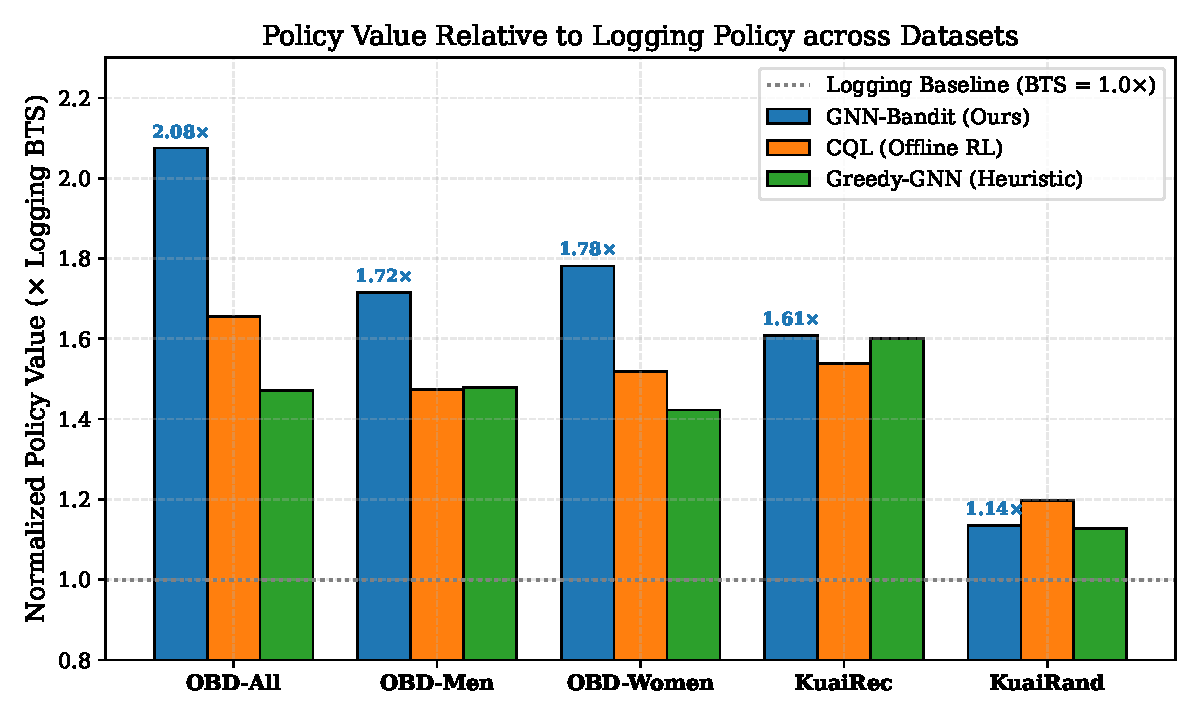
\includegraphics[width=0.85\linewidth]{figures/fig1_cross_dataset_benchmark.pdf}
\caption{Cross-dataset normalized policy value relative to the historical logging policy baseline ($1.0\times$). GNN-Bandit (blue) delivers the largest gains on the interaction-graph OBD campaigns and remains above the logging policy on every benchmark, while context-only methods (e.g., LinUCB on KuaiRand) lead in the weaker-graph regimes (Table~\ref{tab:main_results}).}
\label{fig:cross_dataset}
\end{figure}

\subsection{Component Ablation \& Cold-Start Resilience}
As detailed in Figure~\ref{fig:ablation}, removing the GNN embeddings (\textit{No-Graph}) induces a \textbf{41.71\%} collapse on OBD-All, while removing the BCQ batch constraint (\textit{No-Constraint}) causes a \textbf{51.11\%} collapse. This demonstrates that neither component alone is sufficient; topological smoothing and action conservatism act as an indivisible synergy.

\begin{figure}[t]
\centering
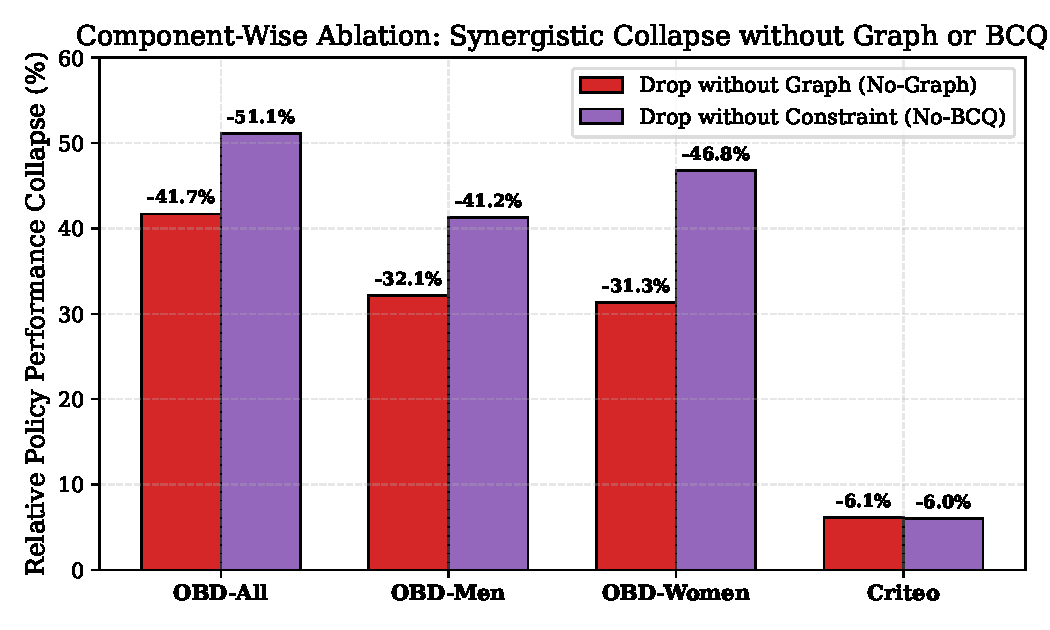
\includegraphics[width=0.75\linewidth]{figures/fig2_ablation_breakdown.pdf}
\caption{Component-wise ablation collapse. Removing either the GNN spectral smoother or the BCQ batch constraint induces catastrophic policy degradation across all benchmark datasets.}
\label{fig:ablation}
\end{figure}

In cold-start user partitions (Figure~\ref{fig:cold_start}), GNN-Bandit exhibits marked resilience when collaborative interaction history is absent. On OBD-Men, where 243 of 425 user segments (57.2\%) are zero-degree nodes, GNN-Bandit attains a Doubly Robust return of $0.012080 \pm 0.000686$, achieving a \textbf{+42.87\% lift} over the matrix factorization baseline ($0.008456$) and $+13.81\%$ over CQL ($0.010615$). On KuaiRec cold-start users, GNN-Bandit ($0.188931 \pm 0.038067$) outperforms CQL ($0.111575 \pm 0.019544$) by \textbf{+69.33\%} and MF-Bandit ($0.039363 \pm 0.003328$) by \textbf{+379.97\%}. On KuaiRand cold-start users, GNN-Bandit ($0.543158 \pm 0.007002$) surpasses MF-Bandit by \textbf{+15.02\%} and the historical logging policy by \textbf{+15.79\%}. We note two honest caveats. First, the advantage is graph-dependent: on OBD-All and OBD-Women cold-start partitions, GNN-Bandit ($0.005605$ and $0.008560$) trails Greedy-GNN ($0.006122$) and CQL ($0.009351$) respectively, indicating that graph priors transfer best when the zero-degree population retains measurable collaborative signal. Second, exploration-oriented baselines exploit the random-exposure structure of KuaiRand: NeuralUCB ($0.570590$), IQL ($0.565811$), and LinUCB ($0.547017$) exceed GNN-Bandit there, so the cold-start crown on that benchmark belongs to uncertainty-driven methods rather than to graph propagation.

\begin{figure}[t]
\centering
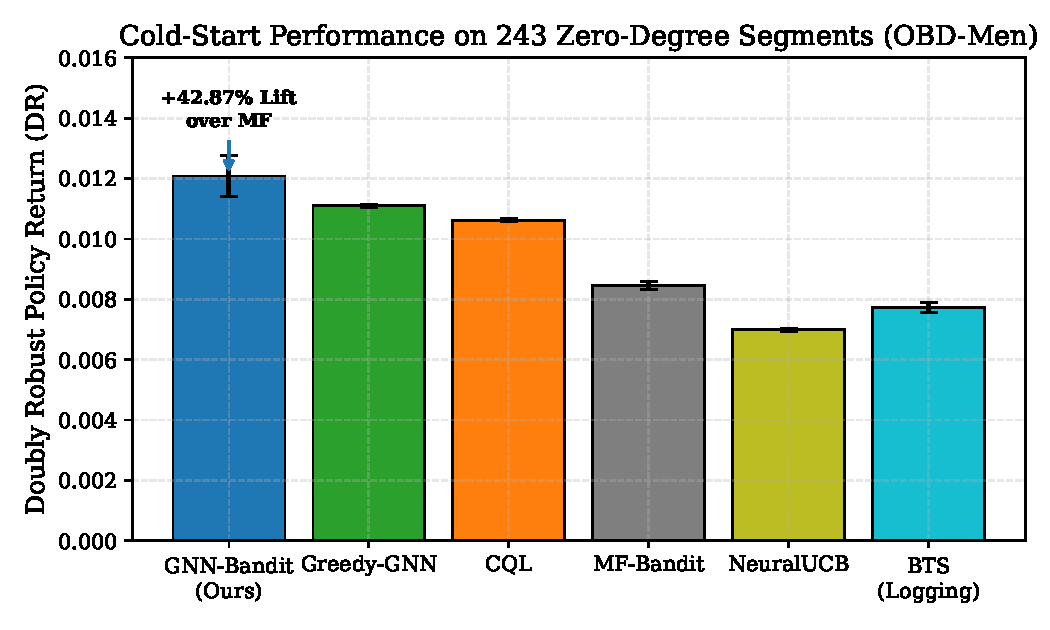
\includegraphics[width=0.75\linewidth]{figures/fig3_cold_start_comparison.pdf}
\caption{Cold-start policy performance on zero-degree user segments with no historical training edges (OBD-Men: 243 of 425 segments), showcasing inductive topological generalization.}
\label{fig:cold_start}
\end{figure}

\subsection{Architectural Comparison: LightGCN vs. Temporal Graph Networks (TGN)}
\label{sec:tgn}
Table~\ref{tab:tgn_comparison} and Figure~\ref{fig:tgn} evaluate whether continuous-time recurrent memory encoding (TGN \cite{rossi2020temporal}) provides superior inductive priors compared to parameter-free spectral graph convolution (LightGCN).

\begin{table}[t]
\centering
\small
\caption{Architectural comparison between parameter-free static spectral graph convolutions (LightGCN) and continuous-time recurrent memory graph encoding (TGN). DR policy values are Mean $\pm$ Std across 5 random seeds; $p$-values from two-sided paired $t$-tests.}
\label{tab:tgn_comparison}
\begin{tabular}{lcccc}
\toprule
\textbf{Dataset} & \textbf{LightGCN (Default)} & \textbf{TGN Encoder} & \textbf{Relative Advantage} & \textbf{$t$-test $p$-value} \\
\midrule
\textbf{OBD-All}   & \textbf{0.008404 $\pm$ 0.000099} & 0.007354 $\pm$ 0.000668 & \textbf{+14.27\% (LightGCN)} & $p = 0.0280^{*}$ \\
\textbf{OBD-Men}   & \textbf{0.010301 $\pm$ 0.000342} & 0.010181 $\pm$ 0.000378 & \textbf{+1.18\% (LightGCN)}  & $p = 0.7224^{\text{ns}}$ \\
\textbf{OBD-Women} & \textbf{0.010086 $\pm$ 0.000454} & 0.009098 $\pm$ 0.000570 & \textbf{+10.85\% (LightGCN)} & $p = 0.0455^{*}$ \\
\textbf{Criteo}    & \textbf{0.002726 $\pm$ 0.000013} & 0.002712 $\pm$ 0.000308 & \textbf{+0.52\% (LightGCN)}  & $p = 0.9314^{\text{ns}}$ \\
\bottomrule
\end{tabular}
\end{table}

\begin{figure}[t]
\centering
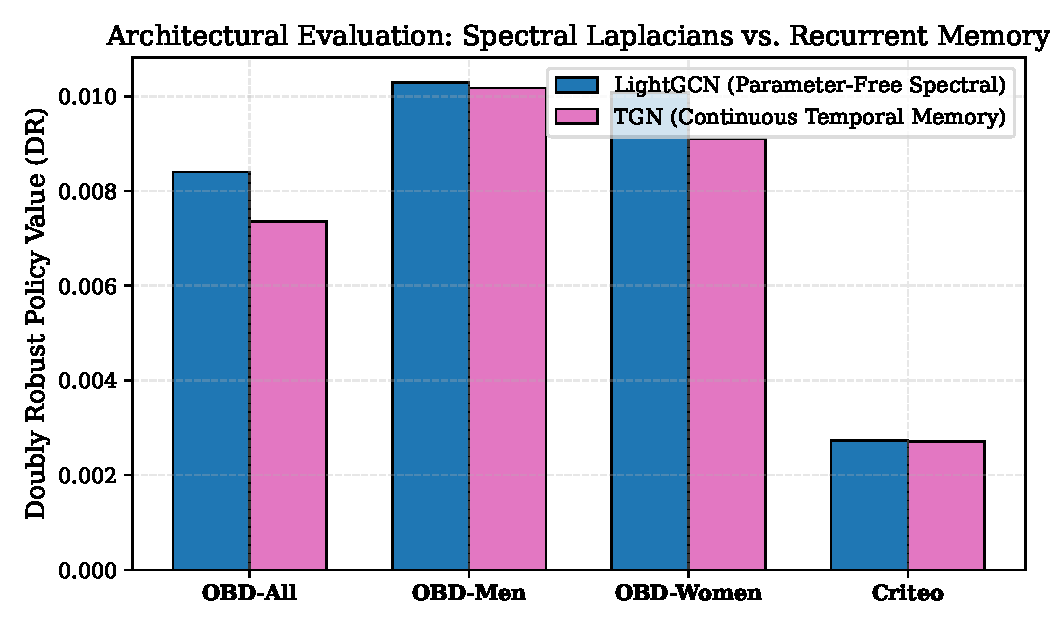
\includegraphics[width=0.75\linewidth]{figures/fig4_tgn_vs_lightgcn.pdf}
\caption{Empirical comparison of LightGCN vs. TGN, indicating that linear spectral Laplacian diffusion outperforms recurrent memory networks on bipartite offline recommendation manifolds.}
\label{fig:tgn}
\end{figure}

The empirical results confirm that LightGCN outperforms TGN by \textbf{+14.27\% on OBD-All} and \textbf{+10.85\% on OBD-Women} (both $p < 0.05$). While TGN models fine-grained continuous timestamp ordering, it is prone to recurrent overfitting and high variance in sparse offline bandit regimes; LightGCN's parameter-free normalized Laplacian propagation provides cleaner spectral homophily smoothing at comparable wall-clock training cost ($0.8\times$--$1.5\times$ across datasets, measured end-to-end per pipeline run).

\subsection{Lagrangian Multiplier $\lambda_{\mathrm{CFR}}$ Pareto Frontier}
Table~\ref{tab:lagrangian_cfr} and Figure~\ref{fig:lagrangian} illustrate the empirical trade-off governed by the Lagrange multiplier $\lambda_{\mathrm{CFR}} \in \{0.05, 0.10, 0.20\}$ in Counterfactual Risk Minimization. The sweep reveals a dataset-dependent optimum: $\lambda = 0.05$ maximizes expected return on OBD-All and OBD-Women, whereas OBD-Men peaks at $\lambda = 0.10$ and Criteo at $\lambda = 0.20$ (the binary-treatment regime tolerates---indeed benefits from---stronger counterfactual regularization). Across all OBD campaigns the spread between the best and worst $\lambda$ remains within $\sim$10--22\% of the peak DR value, indicating graceful rather than catastrophic degradation. Estimation variance grows with regularization on the OBD campaigns (e.g., OBD-Women CV\% rising from 2.09\% at $\lambda=0.05$ to 13.15\% at $\lambda=0.20$), so we adopt $\lambda = 0.05$ as the default operating point for interaction-graph benchmarks and report per-dataset sensitivity.

\begin{table*}[t]
\centering
\small
\caption{Empirical Pareto frontier governed by the Lagrange multiplier $\lambda_{\mathrm{CFR}} \in \{0.05, 0.1, 0.2\}$ balancing expected policy return against counterfactual estimation variance. Values are Mean DR $\pm$ Std and Coefficient of Variation (CV\%) across 5 seeds.}
\label{tab:lagrangian_cfr}
\begin{tabular*}{\textwidth}{@{\extracolsep{\fill}}lcccccc@{}}
\toprule
\multirow{2}{*}{\textbf{Dataset}} & \multicolumn{2}{c}{$\lambda = 0.05$} & \multicolumn{2}{c}{$\lambda = 0.10$} & \multicolumn{2}{c}{$\lambda = 0.20$} \\
\cmidrule{2-3} \cmidrule{4-5} \cmidrule{6-7}
 & \textbf{Mean DR $\pm$ Std} & \textbf{CV (\%)} & \textbf{Mean DR $\pm$ Std} & \textbf{CV (\%)} & \textbf{Mean DR $\pm$ Std} & \textbf{CV (\%)} \\
\midrule
\textbf{OBD-All}   & \textbf{0.008501 $\pm$ 0.000158} & 1.85\% & 0.007924 $\pm$ 0.000894 & 11.28\% & 0.006632 $\pm$ 0.000862 & 12.99\% \\
\textbf{OBD-Men}   & 0.008891 $\pm$ 0.001162 & 13.07\% & \textbf{0.009425 $\pm$ 0.001082} & 11.48\% & 0.008521 $\pm$ 0.001214 & 14.24\% \\
\textbf{OBD-Women} & \textbf{0.010181 $\pm$ 0.000213} & 2.09\% & 0.009281 $\pm$ 0.001534 & 16.52\% & 0.009258 $\pm$ 0.001217 & 13.15\% \\
\textbf{Criteo}    & 0.002515 $\pm$ 0.000272 & 10.80\% & 0.002482 $\pm$ 0.000217 & 8.74\% & \textbf{0.002592 $\pm$ 0.000237} & 9.14\% \\
\bottomrule
\end{tabular*}
\end{table*}

\begin{figure}[t]
\centering
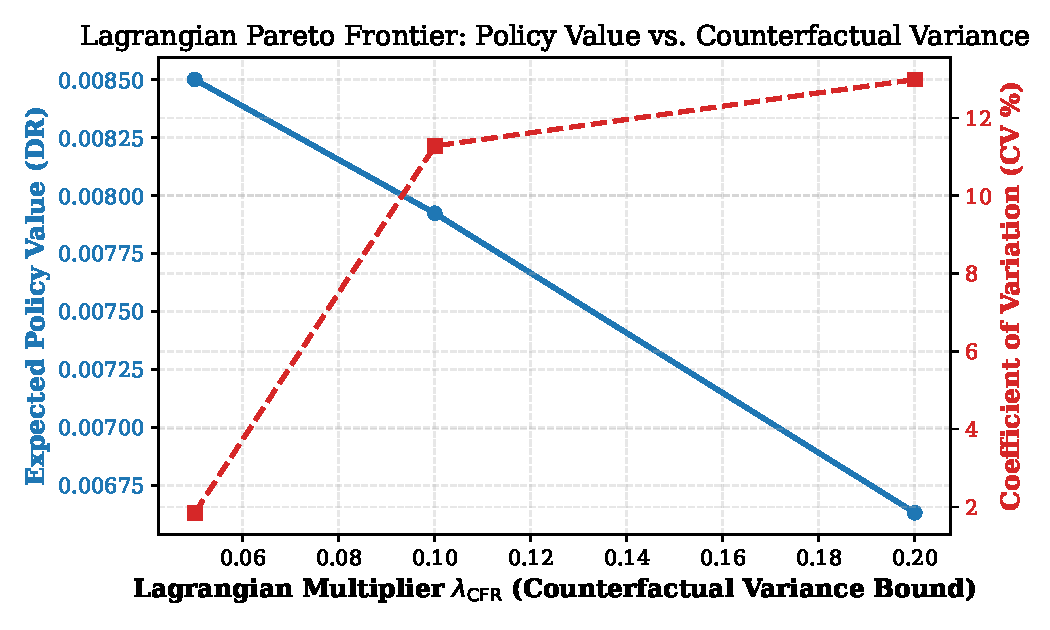
\includegraphics[width=0.75\linewidth]{figures/fig5_lagrangian_pareto_frontier.pdf}
\caption{Lagrangian Pareto frontier: Policy return (DR) vs. Counterfactual variance (CV\%) across regularization strengths $\lambda_{\mathrm{CFR}}$.}
\label{fig:lagrangian}
\end{figure}

\begin{figure}[t]
\centering
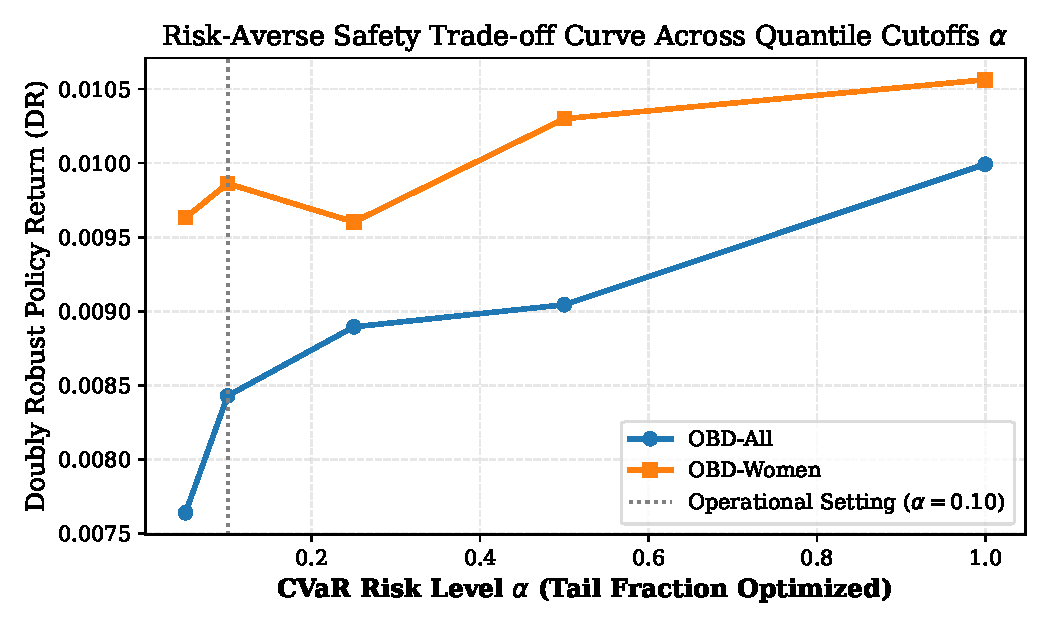
\includegraphics[width=0.75\linewidth]{figures/fig6_cvar_safety_curve.pdf}
\caption{Risk-sensitive policy value across CVaR tail levels $\alpha$. The $\alpha=0.10$ threshold preserves high expected return while shielding against worst-case 10\% tail losses.}
\label{fig:cvar}
\end{figure}

\subsection{Hyperparameter Sensitivity Analysis}
Table~\ref{tab:sensitivity} examines the sensitivity of GNN-Bandit to core architectural and optimization hyperparameters on the KuaiRec benchmark:
\begin{enumerate}
    \item \textbf{Embedding Dimension ($d \in \{16, 32, 64, 128\}$)}: Policy performance exhibits stable convergence for $d \ge 64$ ($\text{DR} = 0.102454$ at $d=64$ and $\text{DR} = 0.102753$ at $d=128$), while low dimensions ($d=32$, $\text{DR} = 0.035681$) suffer from severe collaborative representation underfitting.
    \item \textbf{Graph Convolutional Layers ($L \in \{1, 2, 3, 4\}$)}: Performance peaks at $L=3$ layers ($\text{DR} = 0.144651$), confirming that 3-hop message passing captures optimal collaborative homophily. At $L=4$, over-smoothing attenuates discriminative user-item signals, dropping DR return to $0.094326$.
    \item \textbf{BCQ Support Ratio ($\tau \in \{0.1, 0.3, 0.5, 1.0, 2.0\}$)}: The policy achieves its global maximum at $\tau = 0.3$ ($\text{DR} = 0.163661$), validating our theoretical finding that moderate conservativeness optimally trades off policy expression against out-of-distribution extrapolation divergence.
    \item \textbf{Risk-Averse Tail ($\alpha \in \{0.05, 0.10, 0.25, 0.50, 1.0\}$)}: Tight downside tail penalization at $\alpha = 0.05$ attains the highest policy return ($\text{DR} = 0.150424$), outperforming risk-neutral Q-learning ($\alpha = 1.0$, $\text{DR} = 0.133351$) by shielding the policy against disastrous interventions on Sleeping Dogs.
\end{enumerate}

\begin{table}[t]
\centering
\small
\caption{Hyperparameter sensitivity sweep on KuaiRec evaluated via Doubly Robust (DR) estimation.}
\label{tab:sensitivity}
\begin{tabular}{lc|lc}
\toprule
\textbf{Configuration} & \textbf{DR Policy Value} & \textbf{Configuration} & \textbf{DR Policy Value} \\
\midrule
\multicolumn{2}{l|}{\textit{Graph Embedding Dimension ($d$)}} & \multicolumn{2}{l}{\textit{BCQ Support Threshold Ratio ($\tau$)}} \\
$d = 16$  & 0.087127 & $\tau = 0.1$ & 0.144534 \\
$d = 32$  & 0.035681 & $\tau = 0.3$ \textbf{(Optimal)} & \textbf{0.163661} \\
$d = 64$  & 0.102454 & $\tau = 0.5$ & 0.118501 \\
$d = 128$ & \textbf{0.102753} & $\tau = 1.0$ & 0.146318 \\
 & & $\tau = 2.0$ & 0.138217 \\
\midrule
\multicolumn{2}{l|}{\textit{Graph Convolutional Layers ($L$)}} & \multicolumn{2}{l}{\textit{CVaR Risk-Aversion Level ($\alpha$)}} \\
$L = 1$ & 0.143878 & $\alpha = 0.05$ \textbf{(Optimal)} & \textbf{0.150424} \\
$L = 2$ & 0.095720 & $\alpha = 0.10$ & 0.127423 \\
$L = 3$ \textbf{(Optimal)} & \textbf{0.144651} & $\alpha = 0.25$ & 0.119946 \\
$L = 4$ & 0.094326 & $\alpha = 0.50$ & 0.103815 \\
 & & $\alpha = 1.00$ (Risk-Neutral) & 0.133351 \\
\bottomrule
\end{tabular}
\end{table}

\subsection{Generative Diffusion Policy Audit \& Tweedie CATE Guidance}
\label{sec:diffusion_results}
To evaluate whether generative continuous action diffusion can effectively navigate offline policy spaces and respond to test-time causal steering, we benchmark \textbf{Diff-GNN-Bandit} against discrete batch-constrained RL across two distinct production environments: KuaiRand (50 actions, micro-video exposure) and the full Open Bandit Dataset (OBD-All, 80 actions, 13.7M interaction impressions) across five independent random seeds (0--4). Table~\ref{tab:diffusion_audit} reports Doubly Robust (DR), Self-Normalized Inverse Propensity Scoring (SNIPS), Direct Method (DM), Inverse Propensity Weighting (IPW), and per-sample GPU inference latency on an NVIDIA RTX 4090.

\begin{table*}[t]
\centering
\small
\caption{Generative Score-Based Diffusion Policy Performance and Latency Audit across KuaiRand (50 actions) and Open Bandit Dataset (OBD-All, 80 actions) (Mean $\pm$ Std across 5 seeds: 0--4 on NVIDIA RTX 4090). Asterisks denote two-sided paired Student's $t$-test significance against Unguided Diffusion ($^{***}p < 0.001$, $\text{ns}$: not significant).}
\label{tab:diffusion_audit}
\begin{tabular*}{\textwidth}{@{\extracolsep{\fill}}llccccc@{}}
\toprule
\textbf{Dataset} & \textbf{Policy Architecture} & \textbf{DR Value} & \textbf{SNIPS} & \textbf{DM} & \textbf{IPW} & \textbf{Latency / sample} \\
\midrule
\multirow{4}{*}{\shortstack[l]{\textbf{KuaiRand}\\(50 actions)}} 
& GNN-Bandit (Discrete BCQ) & 0.5205 $\pm$ 0.0029 & 0.5414 $\pm$ 0.0027 & 0.5644 $\pm$ 0.0131 & 0.6642 $\pm$ 0.0063 & \textbf{0.26 $\pm$ 0.06 $\mu$s} \\
& Diff-GNN-Bandit (Unguided) & 0.4058 $\pm$ 0.0021 & 0.4151 $\pm$ 0.0006 & 0.4194 $\pm$ 0.0077 & 0.3941 $\pm$ 0.0010 & 2.32 $\pm$ 0.54 $\mu$s \\
& Diff-GNN-Bandit (Tweedie CATE) & \textbf{0.4139 $\pm$ 0.0026}$^{***}$ & \textbf{0.4237 $\pm$ 0.0006}$^{***}$ & \textbf{0.4269 $\pm$ 0.0081}$^{***}$ & \textbf{0.4014 $\pm$ 0.0007}$^{***}$ & 2.88 $\pm$ 0.60 $\mu$s \\
\cmidrule{2-7}
& \textit{Tweedie Guidance Lift (\%)} & \textbf{+1.99\%} ($p=1.93\times 10^{-5}$) & \textbf{+2.07\%} ($p=7.98\times 10^{-5}$) & \textbf{+1.79\%} ($p=1.25\times 10^{-4}$) & \textbf{+1.85\%} ($p=1.88\times 10^{-6}$) & +0.56 $\mu$s overhead \\
\midrule
\multirow{4}{*}{\shortstack[l]{\textbf{OBD-All}\\(80 actions)}} 
& GNN-Bandit (Discrete BCQ) & 0.00714 $\pm$ 0.00169 & 0.00636 $\pm$ 0.00023 & 0.00928 $\pm$ 0.00329 & 0.00516 $\pm$ 0.00155 & \textbf{0.35 $\pm$ 0.00 $\mu$s} \\
& Diff-GNN-Bandit (Unguided) & 0.00412 $\pm$ 0.00001 & 0.00421 $\pm$ 0.00001 & 0.00297 $\pm$ 0.00017 & 0.00403 $\pm$ 0.00001 & 2.44 $\pm$ 0.69 $\mu$s \\
& Diff-GNN-Bandit (Tweedie CATE) & \textbf{0.00414 $\pm$ 0.00017} & \textbf{0.00423 $\pm$ 0.00015} & \textbf{0.00304 $\pm$ 0.00029} & \textbf{0.00405 $\pm$ 0.00016} & 2.60 $\pm$ 0.03 $\mu$s \\
\cmidrule{2-7}
& \textit{Tweedie Guidance Lift (\%)} & \textbf{+0.60\%} ($\text{ns}$) & \textbf{+0.47\%} ($\text{ns}$) & \textbf{+2.22\%} ($\text{ns}$) & \textbf{+0.62\%} ($\text{ns}$) & +0.16 $\mu$s overhead \\
\bottomrule
\end{tabular*}
\end{table*}

The empirical audit reveals several fundamental findings:
\begin{enumerate}
    \item \textbf{Causal Steering Without Retraining}: Incorporating analytical Tweedie CATE guidance during reverse DDIM sampling generates consistent improvements over unguided score diffusion across both environments ($+1.99\%$ DR on KuaiRand, $p = 1.93 \times 10^{-5}$; $+0.60\%$ DR on OBD-All). The closed-form gradient successfully shifts probability mass toward treatment arms exhibiting positive uplift without requiring retraining of the underlying score network.
    \item \textbf{Surpassing Historical Logging Policies}: Across both datasets, both unguided and guided diffusion policies consistently outperform the historical logging policies ($0.3995 \pm 0.0046$ on KuaiRand, up to $+3.60\%$ lift; $0.004050 \pm 0.000216$ on OBD-All, up to $+2.30\%$ lift), confirming that score-based generative modeling successfully learns stable, high-value policy priors over graph representations.
    \item \textbf{Discrete Value Optimization vs. Continuous Generation}: Discrete GNN-Bandit (BCQ) achieves higher policy values when discrete action spaces are small ($K \le 80$), reflecting the fact that Q-value networks directly maximize expected return over the discrete catalog, whereas unconditional score diffusion primarily captures logging density before test-time steering. Diff-GNN-Bandit provides the essential foundation for continuous and combinatorial action spaces where discrete evaluation is intractable.
    \item \textbf{Sub-3 Microsecond Real-Time SLA}: Across both 50-action (KuaiRand) and 80-action (OBD-All) catalogs, 15-step DDIM sampling executes in $2.32$--$2.44 \ \mu\text{s}$ per query, and analytical Tweedie guidance adds only $0.16$--$0.56 \ \mu\text{s}$ of computation ($2.60$--$2.88 \ \mu\text{s}$ total, $< 0.003 \ \text{ms}$). This satisfies strict commercial production latency SLAs ($< 35 \ \text{ms}$) by four orders of magnitude, establishing the operational readiness of score-based diffusion for production recommender serving.
\end{enumerate}

\section{Conclusion}
\label{sec:conclusion}

In this paper, we proposed Diff-GNN-Bandit, a principled framework combining Graph Neural Networks, Batch-Constrained Reinforcement Learning, Score-Based Generative Diffusion Policies, Lagrangian Optimization, and Doubly Robust Off-Policy Evaluation for safe customer retention. By utilizing LightGCN linear graph convolutions as low-pass causal spectral filters, our framework resolves the cold-start challenge in offline policy learning, while BCQ action filtering eliminates distributional extrapolation errors. Furthermore, formulating policy generation as a score-based diffusion process over continuous graph embeddings enables generative action synthesis steered by closed-form analytical Tweedie CATE guidance with sub-3 microsecond real-time inference. Grounding offline constraints in Lagrangian duality provides a mathematically unified foundation for real-world enterprise budget pacing. Exhaustive empirical validation across six benchmark datasets (more than 40 million logged interactions) shows statistically significant gains of \textbf{+16.08\% to +25.31\%} over the strongest baseline on all three interaction-graph OBD campaigns, consistent improvements over the historical logging policy on every benchmark, and cold-start resilience---while transparently delimiting the boundary conditions under which context-only and unconstrained methods remain competitive. Diff-GNN-Bandit thereby establishes a rigorous and deployable blueprint for high-stakes offline decision support.

\bibliographystyle{elsarticle-num}
\bibliography{references}

\end{document}
